\documentclass{article}
\usepackage{graphicx}
\begin{document}
	\section*{Lsg Vorschlag E I Ü012 Maximilian Maag}
	\section*{Aufgabe 12.1}
	\subsection*{a)}
	Datenwort: 01001011
	Stellen der Prüfbits:$2^0 \land 2^1 \land 2^2 \land2^3$ \\
	Codewort: $--0-100-1011$ \\
	5:0101; 9:1001 11:1011; 12:1100 \\ \\
	 0101 \\
	 1001 \\
	 1011 \\
	 \underline{1100} \\
	 1011 \\ \\
	 Codewort: $100110011011$
	\subsection*{b)}
	Codewort 1: 001010011011 \\
	3: 0011; 5:0101; 8:1000 ;9:1001 ;11:1011 ;12:1100 \\ \\
	0011 \\
	0101 \\
	1000 \\
	1001 \\
	1011 \\
	\underline{1100} \\
	0000 kein Übertragungsfehler\\ \\
	Codewort 2:  110001110110 \\
	1: 0001; 2: 0010; 6: 0110; 7:0111 ; 8:1000; 10:1010; 11:1011 \\ \\
	0001 \\
	0010 \\
	0110 \\
	0111 \\
	1000 \\
	1010 \\
	\underline{1011} \\
	1011 Fehler an der 11. Stelle. \\
	Korrektur: 110001110100
	\section*{Aufgabe 12.2}
	\subsection*{a)}
	Es werden durch den Hamming-Code 8 Paritätsbits und ein zusätzliches, also 9, Bits benötigt.
	\subsection*{b)}
	8 Bits    -5 Paritätsbits     -Mehrkosten von 62,5\% \\
	16 Bits    -6 Paritätsbits    -Mehrkosten von 37,5\% \\
	32 Bits    -7 Paritätsbits    -Mehrkosten von 21,875\% \\
	64 Bits    -8 Paritätsbits    -Mehrkosten von 12,5\% \\
	128 Bits-9 Paritätsbits    -Mehrkosten von 7,03125\% \\
	\section*{Aufgabe 12.3}
	\subsection*{a)}
	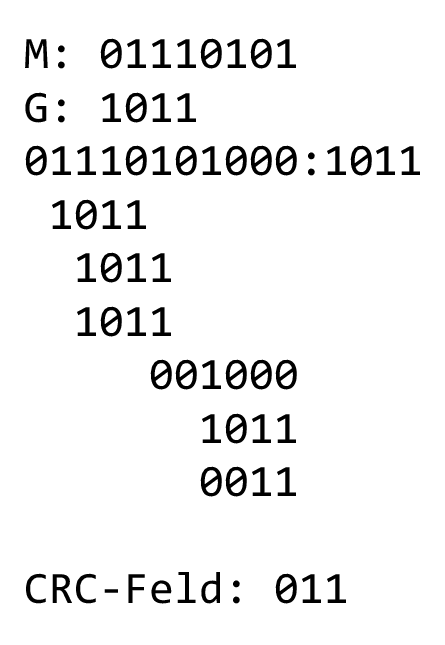
\includegraphics[width=\linewidth]{123a}
	\subsection*{b)}
	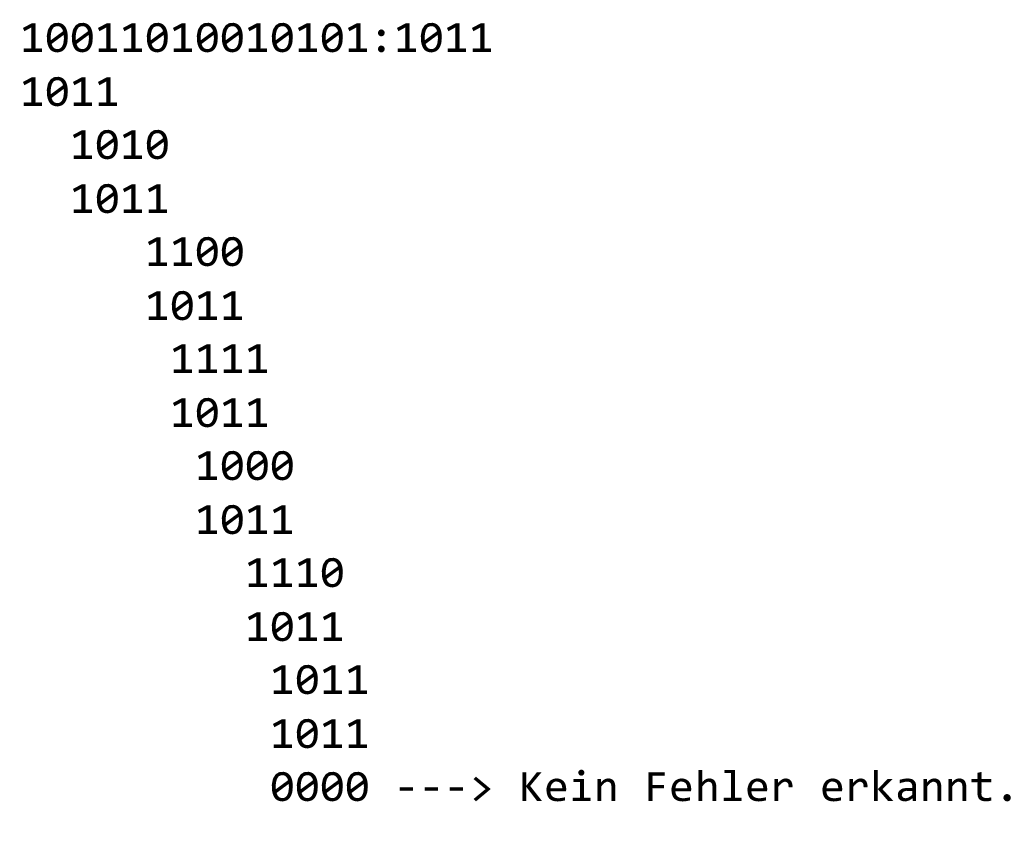
\includegraphics[width=\linewidth]{123b1} \\
	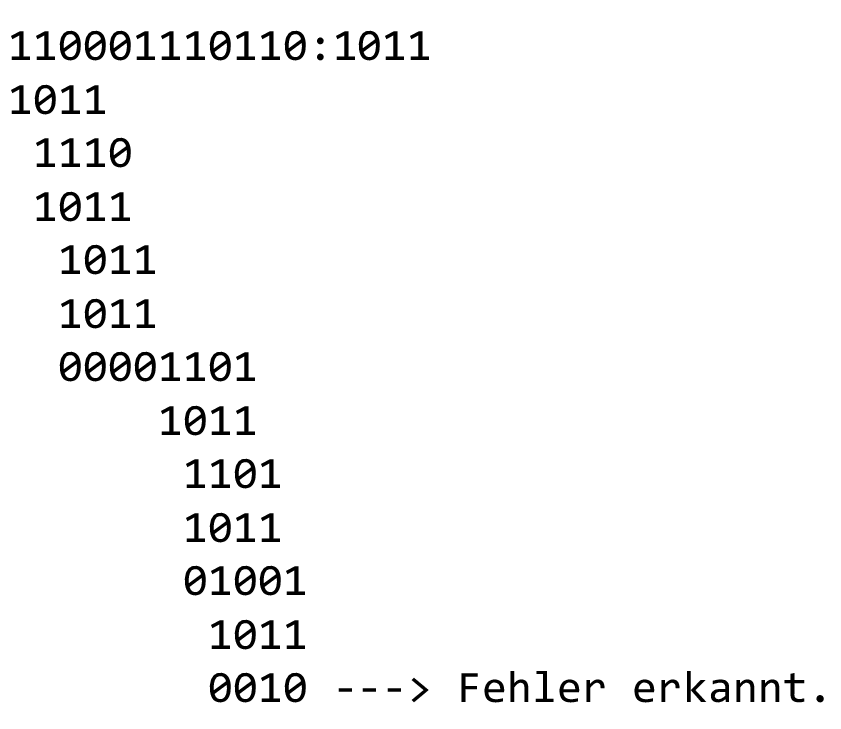
\includegraphics[width=\linewidth]{123b2}
	\subsection*{c)}
	Ein Vielfaches von G(x) auf P(x) addieren um P'(x) zu erhalten. \\
	Bei anschließender Polynomdivision wird kein Fehler erkannt.
	
	\section*{Aufgabe 12.4}
	\subsection*{a)}
	DNF: $S(x_1, x_2, x_3) = (\neg x_1 \land \neg x_2 \land \neg x_3) \lor (x_1 \land \neg x_2 \land \neg x_3) \lor (x_1 \land x_2 \land \neg x_3)$
	\subsection*{b)}
	KNF: $S(x_1, x_2, x_3) = (x_1 \lor x_2 \lor \neg x_3) \land (x_1 \lor \neg x_2 \lor x_3) \land (x_1 \lor \neg x_2 \lor \neg x_3) \land (\neg x_1 \lor x_2 \lor \neg x_3) \land (\neg x_1 \lor \neg x_2 \lor \neg x_3) $
	\section*{Aufgabe 12.5}
	\subsection*{a)}
	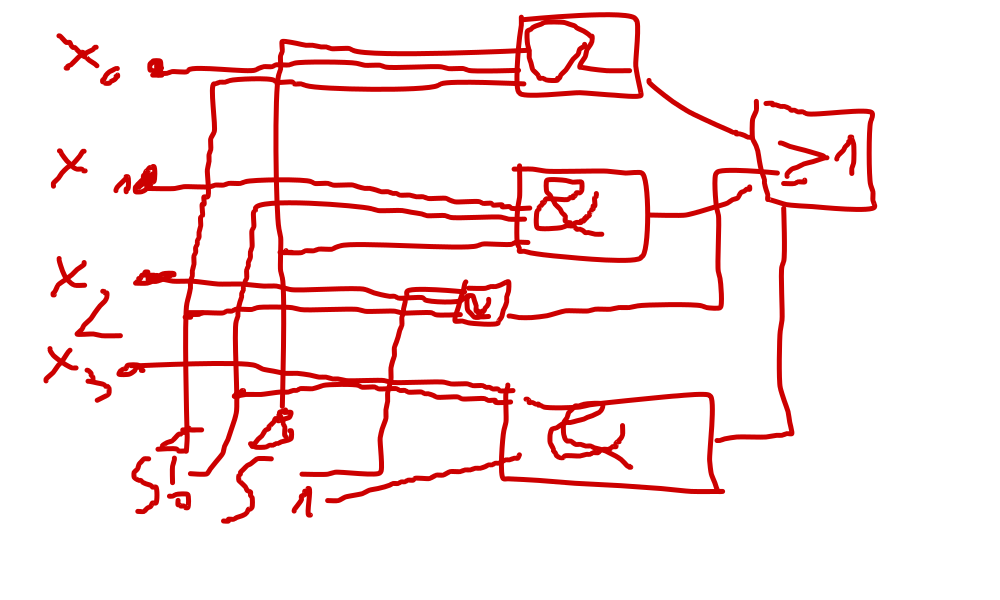
\includegraphics[width=\linewidth]{125a}
	\subsection*{b)}
	Mehrere Signale werden unter Zuhilfenahme von Steuersignalen zu einem Oder Ausgang weitergeleitet. Es handelt sich daher um einen Multiplexer.
\end{document}